% Topic 4 — Async Research Assistant
% Azerbaijani oral-defense deck. Compile twice with XeLaTeX:
%   xelatex -interaction=nonstopmode -halt-on-error slides.tex
% All 19 frames are part of the talk; there is no closing or appendix frame.
% Expanded narration plus per-slide process and term explanations live in
% DEFENSE_RUNBOOK_AZ.md.
\documentclass[aspectratio=169,11pt]{beamer}

\usepackage{fontspec}
\usepackage{tikz}
\usetikzlibrary{arrows.meta,positioning,calc,shapes.geometric}
\usepackage{booktabs}
\usepackage{listings}
\usepackage{array}
\usepackage{graphicx}
\usepackage{xcolor}

\setsansfont{FreeSans}
\setmainfont{FreeSans}
\setmonofont{FreeMono}
\usetheme{default}
\setbeamertemplate{navigation symbols}{}
\setbeamersize{text margin left=7mm,text margin right=7mm}

\definecolor{ink}{HTML}{12263B}
\definecolor{teal}{HTML}{007E86}
\definecolor{orange}{HTML}{D47C2A}
\definecolor{green}{HTML}{26745C}
\definecolor{red}{HTML}{A94C49}
\definecolor{muted}{HTML}{526579}
\definecolor{paper}{HTML}{FAFCFD}
\definecolor{soft}{HTML}{E8F0F4}
\definecolor{aqua}{HTML}{E4F4F3}
\definecolor{amber}{HTML}{FFF1E1}
\definecolor{codebg}{HTML}{F1F5F8}

\setbeamercolor{background canvas}{bg=paper}
\setbeamercolor{normal text}{fg=ink}
\setbeamercolor{frametitle}{fg=ink}
\setbeamerfont{frametitle}{size=\Large,series=\bfseries}
\setbeamertemplate{frametitle}{%
  \vspace{4mm}\hspace{1mm}\insertframetitle\par\vspace{1mm}%
  \hspace{1mm}{\color{teal}\rule{14mm}{1.2pt}}\vspace{1mm}%
}
\setbeamercolor{panel}{bg=soft,fg=ink}
\setbeamercolor{aqua panel}{bg=aqua,fg=ink}
\setbeamercolor{amber panel}{bg=amber,fg=ink}
\setbeamercolor{dark panel}{bg=ink,fg=white}
\newenvironment{panel}{\begin{beamercolorbox}[wd=\linewidth,sep=1.2ex,rounded=true]{panel}}{\end{beamercolorbox}}
\newenvironment{aquapanel}{\begin{beamercolorbox}[wd=\linewidth,sep=1.2ex,rounded=true]{aqua panel}}{\end{beamercolorbox}}
\newenvironment{amberpanel}{\begin{beamercolorbox}[wd=\linewidth,sep=1.2ex,rounded=true]{amber panel}}{\end{beamercolorbox}}
\newenvironment{darkpanel}{\begin{beamercolorbox}[wd=\linewidth,sep=1.2ex,rounded=true]{dark panel}}{\end{beamercolorbox}}
\newcommand{\lead}[1]{{\color{muted}\normalsize #1}\par\vspace{0.75em}}
\newcommand{\tinyref}[1]{{\color{muted}\scriptsize #1}}
\newcommand{\metric}[2]{{\color{teal}\Large\bfseries #1}\par{\small #2}}
\newcommand{\speaker}{ii1ahe}
\setbeamertemplate{footline}{%
  \leavevmode\hbox to\paperwidth{%
    \hspace{7mm}{\color{muted}\scriptsize Topic 4 / \speaker}%
    \hfill{\color{muted}\scriptsize \insertframenumber}\hspace{7mm}}%
  \vspace{2mm}%
}
\lstdefinestyle{project}{
  language=Python,
  basicstyle=\ttfamily\footnotesize,
  keywordstyle=\color{teal}\bfseries,
  stringstyle=\color{orange},
  commentstyle=\color{muted},
  backgroundcolor=\color{codebg},
  frame=single,
  rulecolor=\color{soft},
  framesep=6pt,
  showstringspaces=false,
  columns=fullflexible,
  keepspaces=true,
  breaklines=true
}
\lstdefinestyle{sql}{
  language=SQL,
  basicstyle=\ttfamily\footnotesize,
  keywordstyle=\color{teal}\bfseries,
  backgroundcolor=\color{codebg},
  frame=single,
  rulecolor=\color{soft},
  framesep=6pt,
  columns=fullflexible
}
\tikzset{
  flow/.style={draw=teal,rounded corners=2mm,fill=aqua,align=center,minimum height=12mm,text width=24mm,font=\small},
  source/.style={draw=teal,rounded corners=2mm,fill=white,align=center,minimum height=11mm,text width=26mm,font=\small},
  arr/.style={-Latex,thick,draw=teal}
}

\begin{document}

% 01 — title
{\setbeamercolor{background canvas}{bg=ink}
\setbeamertemplate{footline}{}
\begin{frame}[plain]
  \vspace{7mm}
  {\color{orange}\small AI-ENG-110 \quad SOFTWARE ENGINEERING FINAL PROJECT}\par
  \vspace{9mm}
  {\color{white}\fontsize{29}{33}\selectfont\bfseries Asinxron tədqiqat köməkçisi}\par
  \vspace{4mm}
  {\color{white}\Large Mənbələrdən istinadlı cavabın hazırlanması}\par
  \vspace{9mm}
  {\color{white}\normalsize Wikipedia + arXiv + veb axtarışı \quad $\longrightarrow$ \quad mənbəli cavab}\par
  \vfill
  {\color{white}\small @ii1ahe \quad @Elmin995 \quad @fatimekazimli}\par
  {\color{white!75}\scriptsize github.com/ii1ahe/research-assistant \quad | \quad 18 sentyabr 2026}
\end{frame}}

% 02 — the problem
\begin{frame}{Cavabın mənbələrinin göstərilməsi}
  \lead{Hazırlanan cavabın hansı materiallara əsaslandığı istifadəçiyə göstərilməlidir.}
  \begin{columns}[T,onlytextwidth]
    \column{0.39\linewidth}
      \begin{amberpanel}
        \textbf{Bir sual}\par\vspace{1mm}
        “Fotosintez nədir və əsas mərhələləri hansılardır?”
      \end{amberpanel}
      \vspace{3mm}
      \small Tək axtarış nəticəsindən asılılıq yaradılmaması üçün müxtəlif mənbələrə sorğu göndərilir.
    \column{0.57\linewidth}
      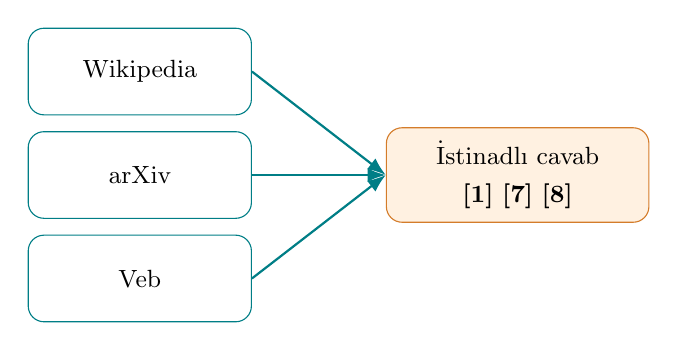
\begin{tikzpicture}[node distance=2mm]
        \node[source] (w) {Wikipedia};
        \node[source,below=of w] (a) {arXiv};
        \node[source,below=of a] (v) {Veb};
        \node[flow,right=17mm of a,text width=31mm,fill=amber,draw=orange] (ans) {İstinadlı cavab\\[1mm]\textbf{[1] [7] [8]}};
        \draw[arr] (w.east) -- (ans.west);
        \draw[arr] (a.east) -- (ans.west);
        \draw[arr] (v.east) -- (ans.west);
      \end{tikzpicture}\par
      \vspace{1mm}
      \tinyref{[1], [7], [8] 18 sentyabr canlı yoxlamasında görünən istinad nömrələridir; bu slayd cavab mətnini təkrar etmir.}
  \end{columns}
\end{frame}

% 03 — contract
\begin{frame}[fragile]{Giriş və çıxış müqaviləsi}
  \lead{Sual və parametrlər qəbul edilir; cavab, mənbələr, status və saxlanma məlumatı qaytarılır.}
  \begin{columns}[T,onlytextwidth]
    \column{0.49\linewidth}
      \textbf{Giriş}\par
      \begin{lstlisting}[style=project]
question: str
sources: tuple[SourceName, ...]
use_cache: bool = True
max_results: int = Field(default=3, ge=1)
      \end{lstlisting}
      \tinyref{Həqiqi sahələr: researcher/models.py, ResearchRequest. CLI limiti sazlamadan götürür.}
    \column{0.49\linewidth}
      \textbf{Çıxış}\par
      \begin{panel}
        \small\textbf{Cavab + nömrəli istinadlar}\par
        Hər mənbənin uğur/boş/xəta vəziyyəti\par
        Sessiyanın saxlanıb-saxlanmaması
      \end{panel}
      \vspace{2mm}
      \begin{aquapanel}
        \small\textbf{Çıxış kodu:} 0 — uğurlu; 1 — cavab yoxdur və ya tələb olunan yazı alınmadı; 2 — giriş/sazlama xətası.
      \end{aquapanel}
  \end{columns}
\end{frame}

% 04 — data/control flow
\begin{frame}{Sorğunun emal mərhələləri}
  \lead{Mənbələrin toplanması ilə yanaşı sıralama, yoxlama və saxlanma qərarları da icra edilir.}
  \vspace{1mm}
  \begin{center}
  \begin{tikzpicture}[node distance=4mm]
    \node[flow] (a) {1\\Giriş və yoxlama};
    \node[flow,right=of a] (b) {2\\Üç mənbəyə sorğu};
    \node[flow,right=of b] (c) {3\\Sıralama və təkrarların silinməsi};
    \node[flow,below=6mm of c] (d) {4\\AI ilə sintez};
    \node[flow,left=of d] (e) {5\\İstinad yoxlaması};
    \node[flow,left=of e] (f) {6\\Sessiya və CLI çıxışı};
    \draw[arr] (a) -- (b);
    \draw[arr] (b) -- (c);
    \draw[arr] (c) -- (d);
    \draw[arr] (d) -- (e);
    \draw[arr] (e) -- (f);
  \end{tikzpicture}
  \end{center}
  \vspace{0mm}
  \begin{aquapanel}
    \small\textbf{Əsas qayda:} sintezdən sonra mənbə sırası dəyişdirilmir; əks halda “[1]” başqa materiala yönələ bilər.
  \end{aquapanel}
\end{frame}

% 05 — architecture
\begin{frame}{Sistemin qatlara bölünməsi}
  \lead{Hər qata ayrıca məsuliyyət verilir; xarici xidmət dəyişdikdə əsas istifadə halı sabit saxlanılır.}
  \begin{center}
  \begin{tikzpicture}[node distance=1.5mm, font=\small]
    \node[flow,text width=36mm] (cli) {CLI / bootstrap\\\scriptsize giriş və resurslar};
    \node[flow,below=of cli,text width=36mm] (core) {ResearchService\\\scriptsize əsas istifadə halı};
    \node[flow,below=5mm of core,text width=39mm] (svc) {Orchestrator + Cache + AIService\\\scriptsize xidmət siyasəti};
    \node[source,left=4mm of svc,text width=30mm,fill=amber,draw=orange] (provided) {verilmiş \texttt{ai/}\\\scriptsize dəyişdirilməyib};
    \node[flow,right=4mm of svc,text width=36mm] (store) {Storage Protocols\\\scriptsize PostgreSQL / yaddaş};
    \draw[arr] (cli) -- (core);
    \draw[arr] (core) -- (svc);
    \draw[arr] (svc) -- (store);
    \draw[arr,dashed] (svc) -- (provided);
  \end{tikzpicture}
  \end{center}
  \vspace{-2mm}
  \tinyref{Qatlı modul monolit: məsuliyyətlər ayrılır, asılılıqlar bootstrap-da birləşdirilir.}
\end{frame}

% 06 — citation integrity
\begin{frame}[fragile]{İstinad nömrələrinin yoxlanması}
  \lead{Cavabın strukturu yoxlanılır; mənbənin iddianı faktiki dəstəkləməsi ayrıca məsələdir.}
  \begin{columns}[T,onlytextwidth]
    \column{0.53\linewidth}
      \textbf{Həqiqi koddan fraqment}\par
      \begin{lstlisting}[style=project]
if not answer.answer.strip():
    raise InvalidAnswerError(
        "the synthesizer returned an empty answer; there is nothing to report",
        source="synthesis",
    )
      \end{lstlisting}
      \tinyref{researcher/validation.py — validate\_answer}
    \column{0.44\linewidth}
      \begin{panel}
        \small\textbf{[1]} $\rightarrow$ siyahıdakı 1-ci mənbə\par
        \textbf{[7]} $\rightarrow$ siyahıdakı 7-ci mənbə\par
        \textbf{[8]} $\rightarrow$ siyahıdakı 8-ci mənbə
      \end{panel}
      \vspace{2mm}
      \small İndeksin müsbət, sərhəd daxilində, təkrarsız və uyğun mənbəyə bağlı olması tələb edilir.
  \end{columns}
\end{frame}

% 07 — concurrency
\renewcommand{\speaker}{Elmin995}
\begin{frame}{Mənbə sorğularının paralel icrası}
  \lead{Şəbəkə gözləmələri üst-üstə salınır; eyni vaxtda icra olunan sorğuların sayı semaforla məhdudlaşdırılır.}
  \begin{columns}[T,onlytextwidth]
    \column{0.49\linewidth}
      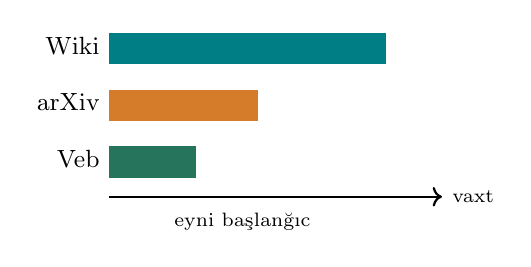
\begin{tikzpicture}[x=0.65cm,y=0.8cm]
        \draw[->,thick] (0,0) -- (6.5,0) node[right,font=\scriptsize] {vaxt};
        \node[left,font=\small] at (0,2.4) {Wiki};
        \node[left,font=\small] at (0,1.5) {arXiv};
        \node[left,font=\small] at (0,0.6) {Veb};
        \fill[teal] (0,2.1) rectangle (5.4,2.6);
        \fill[orange] (0,1.2) rectangle (2.9,1.7);
        \fill[green] (0,0.3) rectangle (1.7,0.8);
        \node[below,font=\scriptsize] at (2.6,-0.1) {eyni başlanğıc};
      \end{tikzpicture}\par
      \vspace{1mm}
      \small Bitmə sırası fərqli ola bilər; nəticələr \texttt{gather} tərəfindən giriş sırası ilə qaytarılır.
    \column{0.48\linewidth}
      \begin{panel}
        \small\textbf{\texttt{asyncio.Semaphore}}\par
        Eyni anda ən çox \texttt{MAX\_PARALLEL\_SOURCES} çağırışının icrasına icazə verilir.
      \end{panel}
      \vspace{2mm}
      \begin{aquapanel}
        \small\textbf{\texttt{asyncio.gather}}\par
        Bütün çağırışlar gözlənilir; bir xətaya görə digər nəticələrin itirilməsi dayandırılır.
      \end{aquapanel}
  \end{columns}
\end{frame}

% 08 — deadlines and degradation
\begin{frame}[fragile]{Mənbə cavab vermədikdə}
  \lead{Hər mənbə ayrıca nəticə kimi qeydə alınır; bir gecikməyə görə digər materiallar itirilmir.}
  \begin{columns}[T,onlytextwidth]
    \column{0.53\linewidth}
      \begin{lstlisting}[style=project,basicstyle=\ttfamily\scriptsize]
async with deadline(
    self._settings.per_source_timeout_seconds,
    source=source.value
):
      \end{lstlisting}
      \small Bu blokda axtarış və təkrar cəhdlər \texttt{execute} tərəfindən idarə edilir.
      \tinyref{researcher/services/ai\_service.py — fetch\_source}
    \column{0.44\linewidth}
      \begin{panel}
        \small Wiki: \textcolor{green}{uğur}\par
        arXiv: \textcolor{red}{vaxt aşımı}\par
        Veb: \textcolor{green}{uğur}
      \end{panel}
      \vspace{2mm}
      \small Qismən nəticə qaytarıla bilər. Vaxt büdcəsinə axtarış və retry daxildir; keş əməliyyatları daxil deyil.
  \end{columns}
\end{frame}

% 09 — retries
\begin{frame}[fragile]{HTTP 429 cavabının emalı}
  \lead{Provayder tərəfindən göstərilən gözləmə müddəti tətbiqin qısa backoff müddətindən üstün tutulur.}
  \begin{columns}[T,onlytextwidth]
    \column{0.50\linewidth}
      \begin{amberpanel}
        \textbf{Müşahidə olunmuş hal: HTTP 429}\par
        Gemini kvotası dolduqda qısa retry cəhdləri eyni vaxt pəncərəsində yenidən rədd edilirdi.
      \end{amberpanel}
      \vspace{3mm}
      \small Gecikmə mesajdan oxunur; orada tapılmadıqda \texttt{Retry-After} başlığı yoxlanılır.
    \column{0.47\linewidth}
      \begin{lstlisting}[style=project,basicstyle=\ttfamily\scriptsize]
retry_after = (
    exc.retry_after_seconds if isinstance(exc, UpstreamRateLimitError) else None
)
      \end{lstlisting}
      \begin{aquapanel}
        \small \textbf{Qayda:} jitterli backoff ilə provayder gecikməsindən daha böyük olan müddət seçilir.
      \end{aquapanel}
  \end{columns}
\end{frame}

% 10 — cache
\begin{frame}{Təkrar sorğuların keşlə azaldılması}
  \lead{Hazır cavab deyil, hər mənbədən alınmış axtarış nəticəsi məhdud müddətə saxlanılır.}
  \begin{columns}[T,onlytextwidth]
    \column{0.51\linewidth}
      \begin{tikzpicture}[node distance=3mm]
        \node[flow,text width=46mm] (k) {5 hissəli keş açarı};
        \node[flow,below=of k,text width=46mm,fill=aqua] (hit) {Təzə qeyd $\rightarrow$ istifadə edilir};
        \node[flow,below=of hit,text width=46mm,fill=amber,draw=orange] (miss) {Qeyd yoxdur $\rightarrow$ canlı axtarış};
        \draw[arr] (k) -- (hit);
        \draw[arr] (hit) -- (miss);
      \end{tikzpicture}
    \column{0.46\linewidth}
      \begin{panel}
        \small\textbf{Açar =} mənbə + normallaşmış sual + provayder + nəticə həddi + sxem versiyası.
      \end{panel}
      \vspace{2mm}
      \small Oxu xətası alındıqda canlı axtarışa keçilir. \texttt{C} və \texttt{C*} sualları hələ qarışdırıla bilər.
  \end{columns}
  \vspace{1mm}
  \tinyref{CacheKey: researcher/models.py; oxu və yazı: researcher/services/orchestrator.py.}
\end{frame}

% 11 — AI boundary
\begin{frame}[fragile]{AI xidməti ilə inteqrasiya}
  \lead{Provayderə aid çağırış və xətalar bir xidmət qatında tətbiqin daxili formatına çevrilir.}
  \begin{columns}[T,onlytextwidth]
    \column{0.52\linewidth}
      \begin{tikzpicture}[node distance=3mm]
        \node[flow,text width=39mm] (core) {ResearchService};
        \node[flow,below=of core,text width=39mm] (svc) {AIService\\\scriptsize retry + deadline + xəta tərcüməsi};
        \node[source,below=of svc,text width=39mm,fill=amber,draw=orange] (ai) {verilmiş \texttt{ai/}\\\scriptsize fetch + synthesize};
        \draw[arr] (core) -- (svc);
        \draw[arr] (svc) -- (ai);
      \end{tikzpicture}
    \column{0.45\linewidth}
      \textbf{Sinxron sintez çağırışı}\par
      \begin{lstlisting}[style=project,basicstyle=\ttfamily\scriptsize]
return await asyncio.to_thread(
    _call_synthesize, question,
    list(materialised), llm
)
      \end{lstlisting}
      \small Çağırış ayrıca thread-də icra edilir; timeout baş verdikdə thread dərhal dayandırılmır.
  \end{columns}
  \vspace{1mm}
  \tinyref{Wikipedia fulltext axtarışı MediaWiki-yə birbaşa gedir; verilmiş \texttt{ai/} dəyişdirilməyib.}
\end{frame}

% 12 — storage
\renewcommand{\speaker}{fatimekazimli}
\begin{frame}[fragile]{Məlumatların PostgreSQL-də saxlanması}
  \lead{Mənbə keşi və tamamlanmış tədqiqat sessiyası ayrı məqsədlər üçün saxlanılır.}
  \begin{columns}[T,onlytextwidth]
    \column{0.49\linewidth}
      \begin{aquapanel}
        \textbf{source\_cache}\par
        \small Açarın 5 hissəsi + JSONB məzmun + bitmə vaxtı.
      \end{aquapanel}
      \vspace{2mm}
      \begin{panel}
        \scriptsize \textbf{Əsas açar:} source + query + provider + max\_results + schema\_version
      \end{panel}
    \column{0.48\linewidth}
      \begin{panel}
        \textbf{research\_sessions}\par
        \small UUID + vaxt + status + sual + bütün nəticəni saxlayan JSONB.
      \end{panel}
      \vspace{2mm}
      \small Eyni müqavilənin PostgreSQL və yaddaş variantında qorunması \texttt{SourceCache} və \texttt{SessionRepository} Protocol-ları ilə təmin edilir.
  \end{columns}
  \vspace{2mm}
  \tinyref{migrations/001\_initial\_schema.sql; researcher/storage/interfaces.py və postgres.py.}
\end{frame}

% 13 — runtime/deployment
\begin{frame}{Tətbiqin işə salınması}
  \lead{Sazlama və resurslar bootstrap mərhələsində yaradılır, çıxış zamanı bağlantılar bağlanır.}
  \begin{center}
  \begin{tikzpicture}[node distance=5mm]
    \node[flow,text width=35mm] (cli) {CLI\\\scriptsize \texttt{python -m researcher ask}};
    \node[flow,right=of cli,text width=35mm] (boot) {Bootstrap\\\scriptsize sazlama + resurslar};
    \node[flow,right=of boot,text width=35mm] (app) {ResearchService\\\scriptsize sorğu və nəticə};
    \draw[arr] (cli) -- (boot);
    \draw[arr] (boot) -- (app);
    \node[source,below=7mm of boot,text width=35mm] (pg) {PostgreSQL\\\scriptsize Docker Compose və ya ayrıca};
    \draw[arr] (boot) -- (pg);
  \end{tikzpicture}
  \end{center}
  \vspace{-1mm}
  \begin{amberpanel}
    \small \textbf{İşləmə şərtləri:} canlı cavab üçün internet və API açarı tələb edilir. PostgreSQL qurulmadıqda bazasız rejim istifadə olunur. \texttt{PERSIST\_SESSIONS=false} yalnız sessiya yazısını söndürür.
  \end{amberpanel}
\end{frame}

% 14 — tests
\begin{frame}{Test nəticələri və onların sərhədi}
  \lead{Tətbiqin idarə edilən davranışı yoxlanılır; xarici provayderin daimi əlçatanlığı bu nəticələrlə təsdiqlənmir.}
  \begin{columns}[T,onlytextwidth]
    \column{0.31\linewidth}
      \begin{aquapanel}\metric{380}{test; PostgreSQL olduqda hamısı keçirilir}\end{aquapanel}
    \column{0.31\linewidth}
      \begin{aquapanel}\metric{96\%}{\texttt{researcher/} sətir əhatəsi}\end{aquapanel}
    \column{0.31\linewidth}
      \begin{aquapanel}\metric{16/16}{verilmiş \texttt{ai/} smoke testləri}\end{aquapanel}
  \end{columns}
  \vspace{5mm}
  \begin{panel}
    \small \textbf{Test quruluşu:} AI və HTTP cavabları saxtalaşdırılır; internet çıxışı fixture ilə bloklanır; PostgreSQL olmadıqda 8 inteqrasiya testi səbəb göstərilərək buraxılır.
  \end{panel}
  \vspace{2mm}
  \tinyref{Əhatə faizi cavabın fakt doğruluğu faizi deyil.}
\end{frame}

% 15 — benchmark
\begin{frame}{Benchmark nəticələri}
  \lead{Mənbə toplama mərhələsi sürətlənir; ümumi vaxtın böyük hissəsi AI sintezinə sərf edilir.}
  \begin{columns}[T,onlytextwidth]
    \column{0.54\linewidth}
      \textbf{Beş sual üzrə mərhələ cəmi}\par\vspace{3mm}
      \small Axtarış, ardıcıl \quad 4,83 s\par
      {\color{orange}\rule{49mm}{4mm}}\par\vspace{2mm}
      \small Axtarış, paralel \quad 2,89 s\par
      {\color{teal}\rule{29mm}{4mm}}\par\vspace{3mm}
      \small Bütöv icra \quad 43,45 s $\rightarrow$ 43,33 s
    \column{0.43\linewidth}
      \begin{aquapanel}
        \metric{1,67$\times$}{mənbə toplama sürəti}
      \end{aquapanel}
      \vspace{2mm}
      \begin{amberpanel}
        \metric{1,00$\times$}{bütöv icra sürəti}
      \end{amberpanel}
  \end{columns}
  \vspace{3mm}
  \tinyref{12 sentyabr artefaktı: 5 sual, 3 mənbə, keş söndürülüb, 0 mənbə xətası; model gemini-3.6-flash. 10 s sualarası fasilə mərhələ vaxtlarına daxil deyil.}
\end{frame}

% 16 — reproduction
\begin{frame}{Təmiz mühitdə reproduksiya}
  \lead{Tətbiqin başqa mühitdə qurulması və test edilməsi ilə reproduksiya qabiliyyəti yoxlanılır.}
  \begin{columns}[T,onlytextwidth]
    \column{0.49\linewidth}
      \begin{panel}
        \textbf{Aparılmış yoxlama}\par\vspace{2mm}
        \small GitHub Codespaces-də təmiz klon yaradılıb, Docker image qurulub, smoke və tam test dəstləri icra edilib.
      \end{panel}
      \vspace{2mm}
      \small Həmin köhnə commitdə 349 test keçdi, 7 baza testi şəbəkə səbəbindən buraxıldı.
    \column{0.48\linewidth}
      \begin{amberpanel}
        \textbf{Qeydə alınmış problem}\par\vspace{2mm}
        \small Əlçatan olmayan baza üçün bağlantı cəhdi təxminən 60 saniyə davam edirdi.
      \end{amberpanel}
      \vspace{2mm}
      \small Sonrakı düzəlişdə bağlantının açılmasına 10 saniyəlik hədd verilib; bu, ayrıca SQL sorğusunun həddi deyil.
  \end{columns}
  \vspace{3mm}
  \tinyref{Sübut: artefacts/reproduction-codespaces-bfec78.txt. Orada canlı AI cavabı yoxlanmamışdı.}
\end{frame}

% 17 — live run
\renewcommand{\speaker}{ii1ahe}
\begin{frame}{Canlı icranın nəticəsi}
  \lead{18 sentyabrda real mənbələrdən material toplanıb, istinadlı cavab yaradılıb və sessiya PostgreSQL-də saxlanılıb.}
  \begin{columns}[T,onlytextwidth]
    \column{0.55\linewidth}
      \begin{panel}
        \textbf{Fotosintez sualı}\par\vspace{2mm}
        \small 3 mənbə $\rightarrow$ 8 təkrarsız nəticə $\rightarrow$ istinadlı cavab\par
        \small Qeydə alınmış istinadlar: \textbf{[1], [7], [8]}\par
        \small Sessiya: \textcolor{green}{PostgreSQL-də saxlanılıb}
      \end{panel}
    \column{0.42\linewidth}
      \begin{aquapanel}\metric{1,51 s}{mənbə toplama}\end{aquapanel}
      \vspace{2mm}
      \begin{aquapanel}\metric{3,46 s}{AI sintezi}\end{aquapanel}
      \vspace{2mm}
      \small İki mərhələnin cəmi: \textbf{4,97 s}.
  \end{columns}
  \vspace{1mm}
  \tinyref{18 sentyabr / gemini-3.1-flash-lite / tək icra; beş suallıq benchmark deyil.}
\end{frame}

% 18 — limitations
\begin{frame}{Mövcud məhdudiyyətlər}
  \lead{Test və istinad yoxlamaları cavabın faktiki doğruluğuna zəmanət vermir.}
  \begin{columns}[T,onlytextwidth]
    \column{0.48\linewidth}
      \begin{amberpanel}
        \textbf{Məzmun}\par
        \small Düzgün nömrəli istinadla yanlış iddia təqdim edilə bilər. İddia–mənbə uyğunluğu ayrıca yoxlanılmalıdır.
      \end{amberpanel}
      \vspace{2mm}
      \begin{amberpanel}
        \textbf{Keş açarı}\par
        \small \texttt{C} və \texttt{C*} hələ toqquşa bilər; versiya 1 köhnə qeydləri ayırmır.
      \end{amberpanel}
    \column{0.48\linewidth}
      \begin{amberpanel}
        \textbf{Baza gözləməsi}\par
        \small SQL timeout var, lakin pool-dan bağlantı almaq ayrıca hədlənmir.
      \end{amberpanel}
      \vspace{2mm}
      \begin{amberpanel}
        \textbf{Sintez thread-i}\par
        \small Coroutine vaxtı bitəndə xarici çağırış bir müddət daha işləyə bilər.
      \end{amberpanel}
  \end{columns}
\end{frame}

% 19 — contributions
\renewcommand{\speaker}{hər üç üzv}
\begin{frame}{Töhfələr və AI alətlərindən istifadə}
  \lead{Təqdimat bölgüsü ilə kod müəllifliyi ayrılır; faktiki işlər repo tarixçəsi və töhfə bəyanatında göstərilir.}
  \begin{columns}[T,onlytextwidth]
    \column{0.31\linewidth}
      \begin{panel}
        \textbf{ii1ahe}\par\vspace{1mm}
        \small Tətbiq, testlər, infrastruktur və sənədlərin əsas hissəsi hazırlanıb.
      \end{panel}
    \column{0.31\linewidth}
      \begin{panel}
        \textbf{Elmin995}\par\vspace{1mm}
        \small PR \#11 və \#12 üzrə review aparılıb və qeydlər verilib.
      \end{panel}
    \column{0.31\linewidth}
      \begin{panel}
        \textbf{fatimekazimli}\par\vspace{1mm}
        \small Təmiz klon reproduksiyası aparılıb və nəticə artefaktı hazırlanıb.
      \end{panel}
  \end{columns}
  \vspace{5mm}
  \begin{aquapanel}
    \small \textbf{Açıqlama:} Claude-dan kod, test və ilkin sənəd qaralamalarında; OpenAI Codex-dən audit, düzəliş, canlı yoxlama və təqdimatın hazırlanmasında istifadə olunub. Faktiki rollar imzalı töhfə sənədində göstərilib.
  \end{aquapanel}
\end{frame}

\end{document}
